% !TEX TS-program = pdflatex
% !TEX encoding = UTF-8 Unicode

% This is a simple template for a LaTeX document using the "article" class.
% See "book", "report", "letter" for other types of document.

\documentclass[20pt]{article} % use larger type; default would be 10pt

\usepackage[utf8]{inputenc} % set input encoding (not needed with XeLaTeX)

%%% Examples of Article customizations
% These packages are optional, depending whether you want the features they provide.
% See the LaTeX Companion or other references for full information.

%%% PAGE DIMENSIONS
\usepackage{geometry} % to change the page dimensions
\geometry{a4paper} % or letterpaper (US) or a5paper or....
% \geometry{margin=2in} % for example, change the margins to 2 inches all round
% \geometry{landscape} % set up the page for landscape
%   read geometry.pdf for detailed page layout information

\usepackage{graphicx} % support the \includegraphics command and options

% \usepackage[parfill]{parskip} % Activate to begin paragraphs with an empty line rather than an indent

%%% PACKAGES
\usepackage{booktabs} % for much better looking tables
\usepackage{array} % for better arrays (eg matrices) in maths
\usepackage{paralist} % very flexible & customisable lists (eg. enumerate/itemize, etc.)
\usepackage{verbatim} % adds environment for commenting out blocks of text & for better verbatim
%\usepackage{subfig} % make it possible to include more than one captioned figure/table in a single float
\usepackage{mathtools}
\usepackage{graphicx} % supports images in latex
% These packages are all incorporated in the memoir class to one degree or another...

\usepackage{graphicx}
\usepackage{subcaption}

%%% Other stuff
\DeclarePairedDelimiter\ceil{\lceil}{\rceil}
\DeclarePairedDelimiter\floor{\lfloor}{\rfloor}

%%% HEADERS & FOOTERS
\usepackage{fancyhdr} % This should be set AFTER setting up the page geometry
\pagestyle{fancy} % options: empty , plain , fancy
\renewcommand{\headrulewidth}{0pt} % customise the layout...
\lhead{}\chead{}\rhead{}
\lfoot{}\cfoot{\thepage}\rfoot{}

%%% SECTION TITLE APPEARANCE
\usepackage{sectsty}
\allsectionsfont{\sffamily\mdseries\upshape} % (See the fntguide.pdf for font help)
% (This matches ConTeXt defaults)

%%% ToC (table of contents) APPEARANCE
\usepackage[nottoc,notlof,notlot]{tocbibind} % Put the bibliography in the ToC
\usepackage[titles,subfigure]{tocloft} % Alter the style of the Table of Contents
\renewcommand{\cftsecfont}{\rmfamily\mdseries\upshape}
\renewcommand{\cftsecpagefont}{\rmfamily\mdseries\upshape} % No bold!

%%% Code syntax highliting
\usepackage{listings}
%\begin{lstlisting}[language=java]
%\end{lstlisting}

%%% graphics path \graphicspath{{./HW5}}

%%% END Article customizations

%%% nice things to keep around

% \noindent\rule{2cm}{0.4pt} 
%%% puts a small horizontal line

% \mathcal{O} 
%%% big O notation

%\begin{figure}[!htbp]
%  	\centering
%   	\begin{subfigure}[p]{0.5\linewidth}
%    	\includegraphics[width=\linewidth]{}
%   	\end{subfigure}
%\end{figure} 

%%% The "real" document content comes below...

\title{Computational Statistics Homework 3}
\author{Liam Dillingham}
%\date{} % Activate to display a given date or no date (if empty),
         % otherwise the current date is printed 

\begin{document}
\maketitle

\section{Question 1} 
Implement the Gibbs sampler from the assignment sheet for generating bivariate samples from the join density $(s, \theta)$. 
\subsection{Draw the trace plot for the $s^{(i)}$ samples}
\begin{figure}[!htbp]
  	\centering
   	\begin{subfigure}[p]{0.9\linewidth}
    	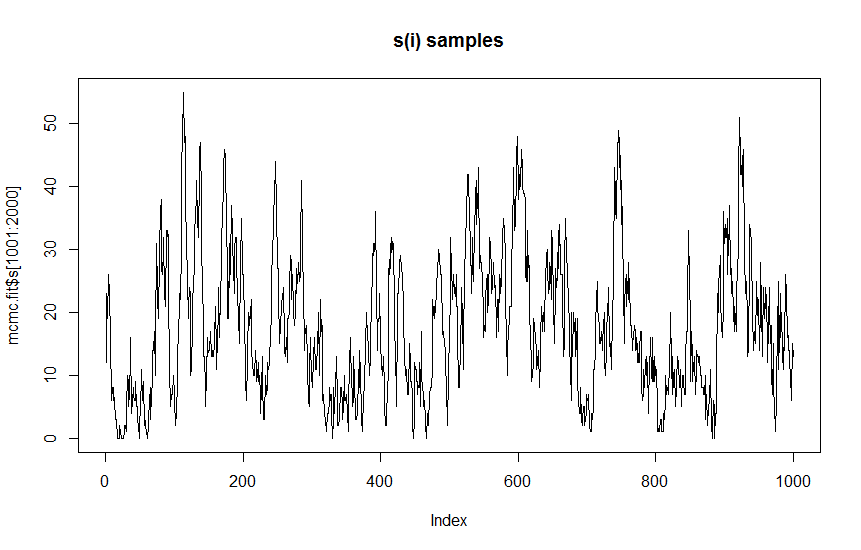
\includegraphics[width=\linewidth]{./figures/hw3-01.png}
   	\end{subfigure}
\end{figure} 
\newpage
\subsection{Draw the traceplot for the $\theta^{(i)}$ samples}
\begin{figure}[!htbp]
  	\centering
   	\begin{subfigure}[p]{0.9\linewidth}
    	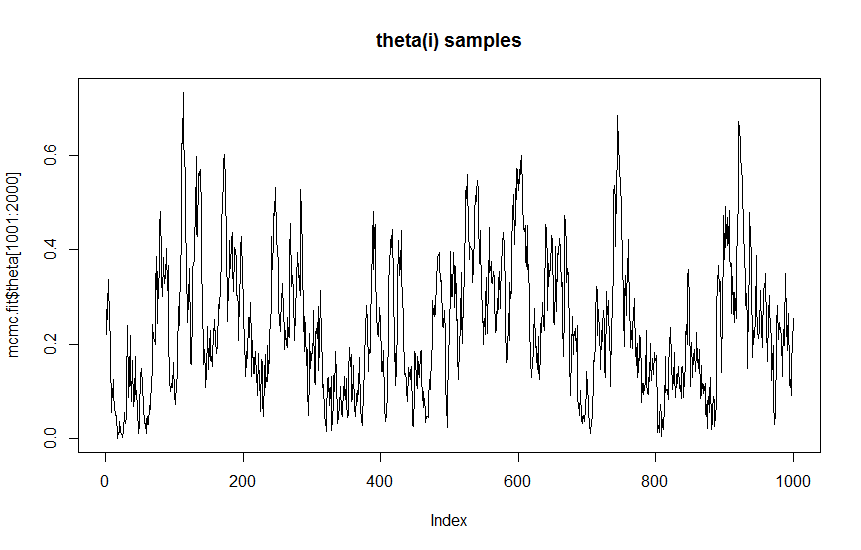
\includegraphics[width=\linewidth]{./figures/hw3-02.png}
   	\end{subfigure}
\end{figure} 
\subsection{Draw the histogram for the $s^{(i)}$ samples}
\begin{figure}[!htbp]
  	\centering
   	\begin{subfigure}[p]{0.9\linewidth}
    	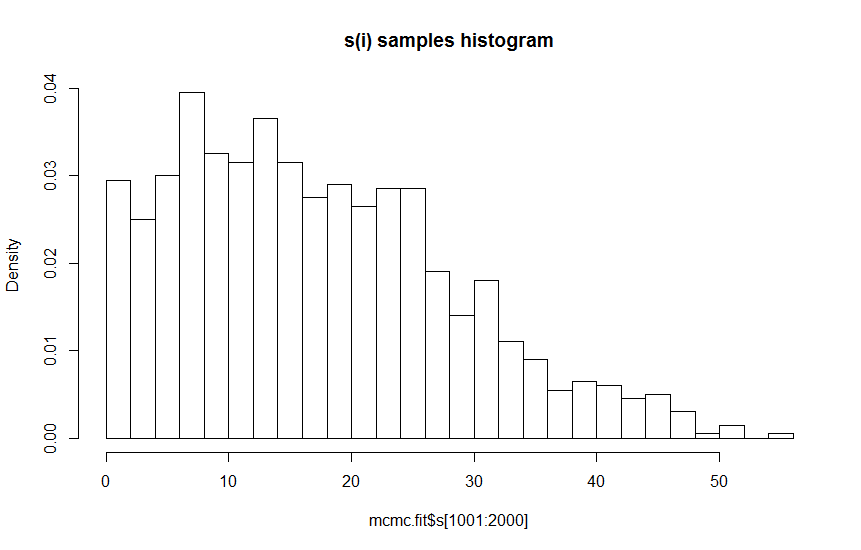
\includegraphics[width=\linewidth]{./figures/hw3-03.png}
   	\end{subfigure}
\end{figure} 
\subsection{Estimate the posterior median of $\theta$ based on the samples drawn. Is it close to the maximum likelihood estimate of $s/n$?}
From the problem description, it states that the maximum likelihood estimate of theta, $\hat{\theta}_{mle}$, is equal to $s/n = 74/16 = 0.2162162$.  By calculating the post burn-in simulation of our Gibbs sampler, we achieve a median value of $0.2198654$
\subsection{How sensitive is the posterior median to the choice of initial values?}

\section{Question 2}
Implement the Gibbs sampler from before but treat $n$ as an unknown paramter as well with a Poisson prior on $n$, i.e. $\pi(n) = \text{Poisson}(\lambda)$.  Assume $(\lambda = 64)$.
\\ \noindent\rule{2cm}{0.4pt} \\


\end{document}




